% Standalone version for TikZ annotation tuning
% Compile: pdflatex fig_servo_standalone.tex
\documentclass[border=5pt]{standalone}
\usepackage{tikz}
\usetikzlibrary{arrows.meta, calc}
\usepackage{amsmath}
\usepackage{graphicx}
\graphicspath{{./}}

\begin{document}
\begin{tikzpicture}[
  every node/.style={font=\small},
  lbl/.style={font=\footnotesize},
  dimarr/.style={{Stealth[length=3pt]}-{Stealth[length=3pt]}, thin, black},
]
  \node[anchor=south west, inner sep=0] (img) at (0,0)
    {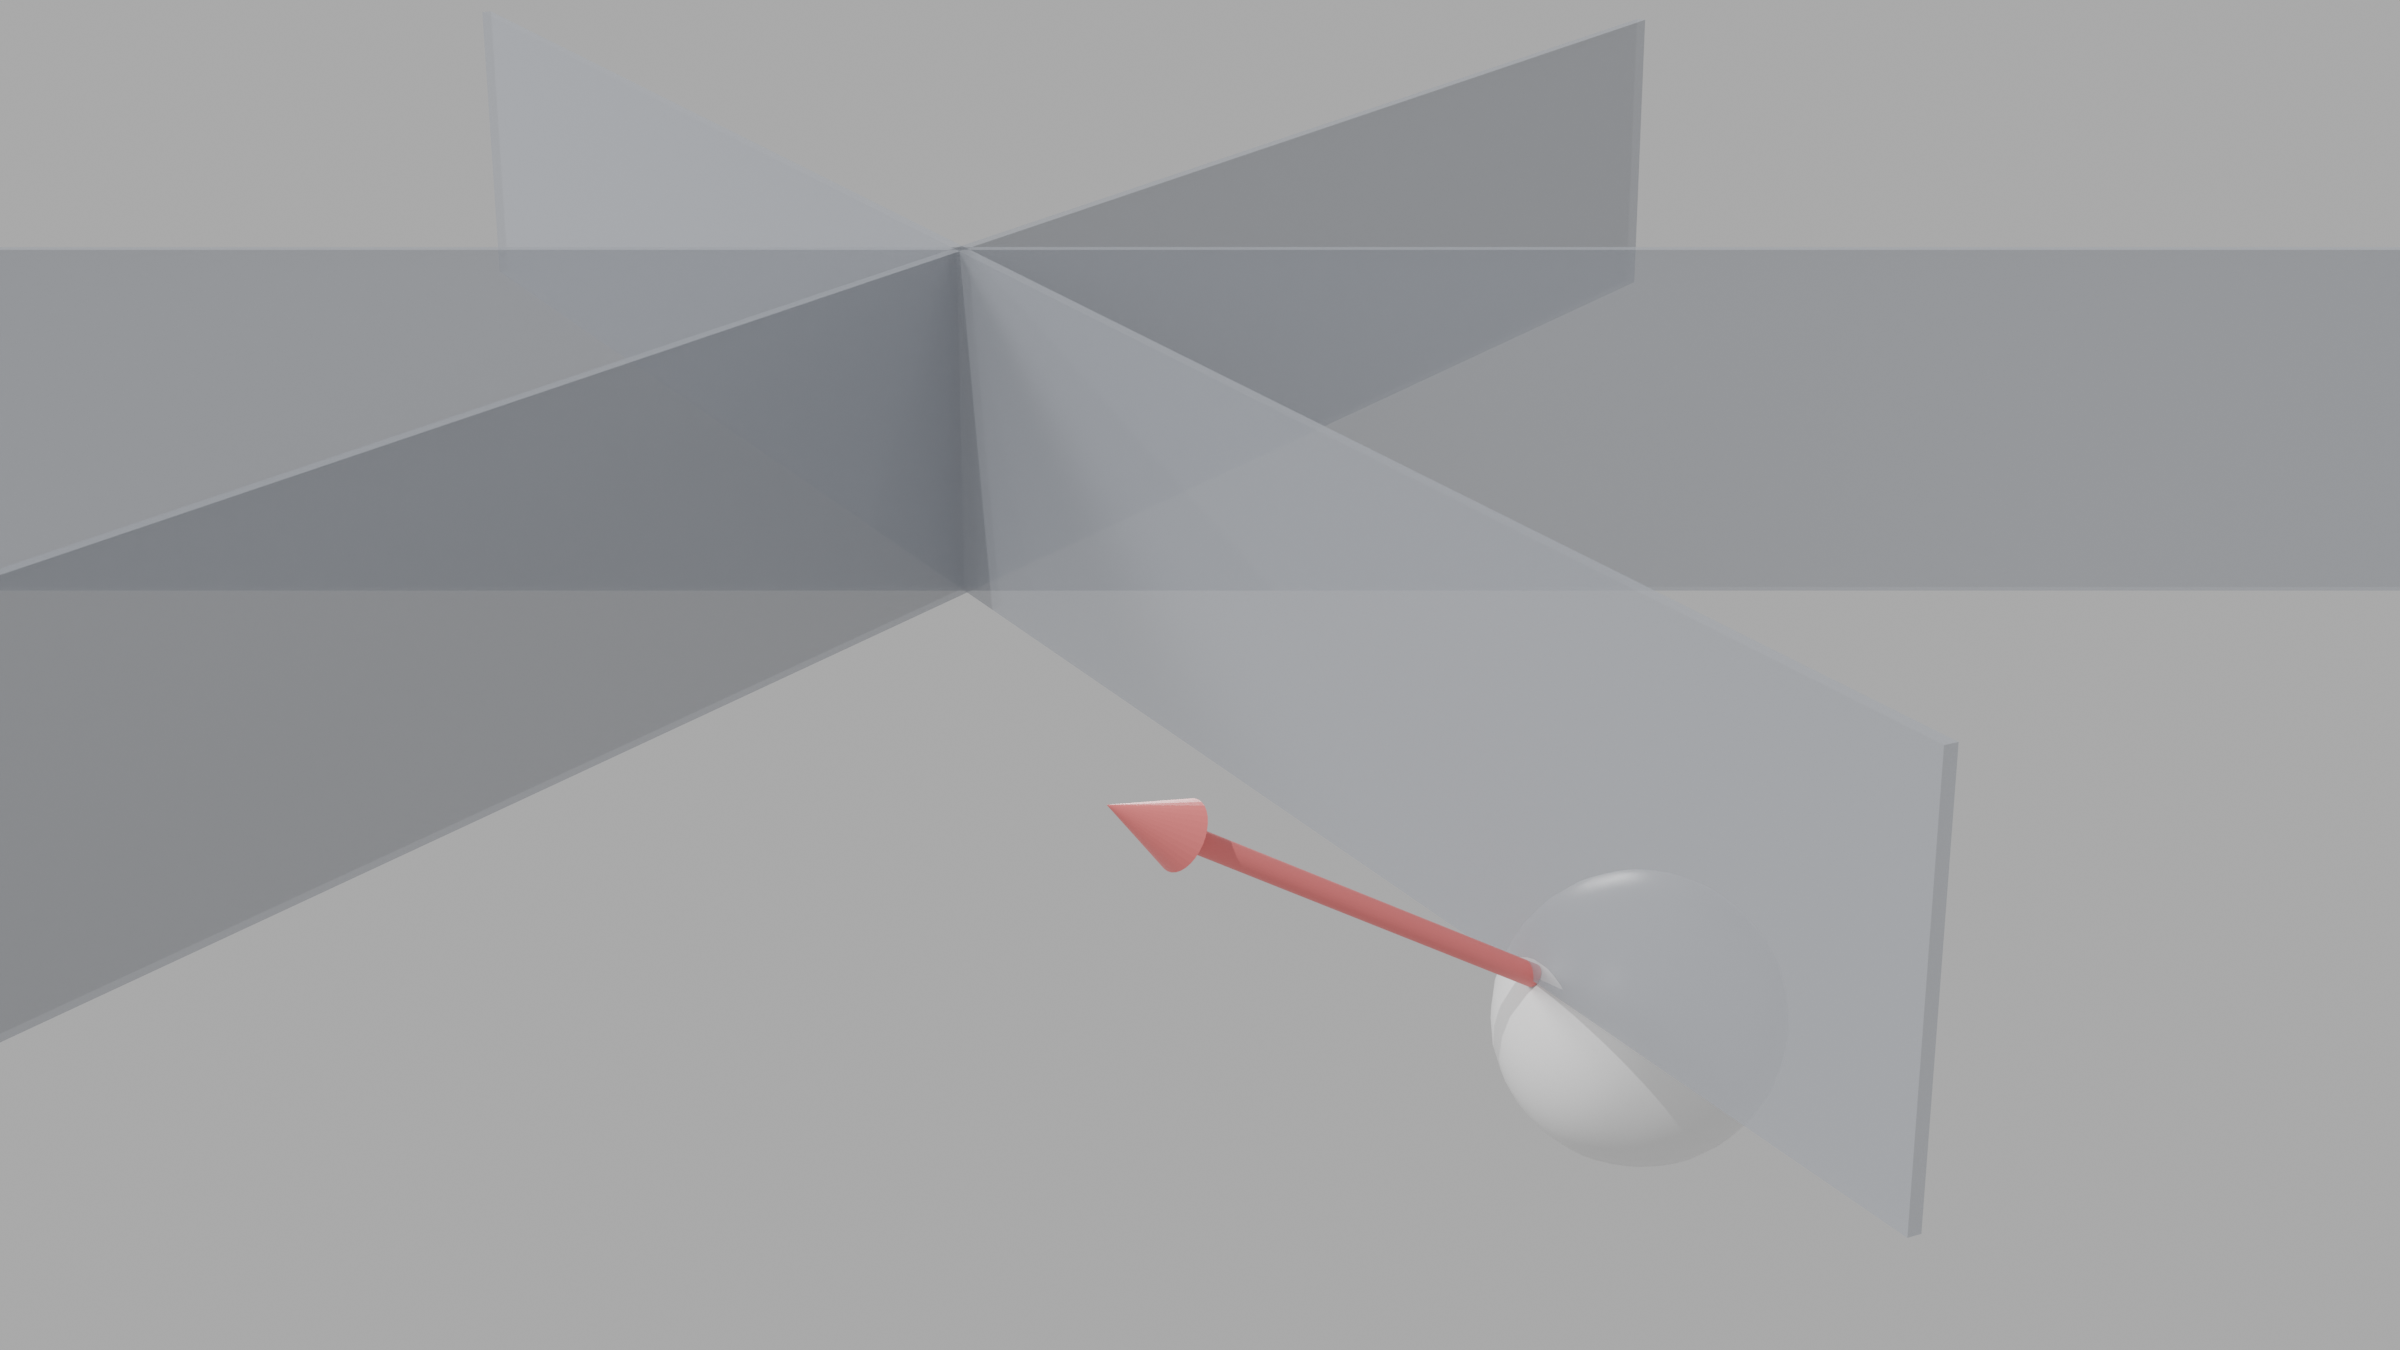
\includegraphics[width=10cm]{servo_torsional_contact_geometry.png}};
  \begin{scope}[
    x={(img.south east)},
    y={(img.north west)},
  ]
    % --- Contact point (arrow tail, at ball-blade interface) ---
    \coordinate (CP) at (0.646, 0.276);

    % --- Arrowhead tip ---
    \coordinate (AH) at (0.45, 0.4);

    % --- HCA center axis (where blades converge) ---
    \coordinate (RA) at (0.4, 0.80);
    \coordinate (RA_h) at (0.4, 0.56);

    % --- Contact normal label n ---
    \node[lbl, red!70!black, above right] at (0.46, 0.4) {$\mathbf{n}$};

    % --- Horizontal reference line (dashed) at contact point ---
    \draw[densely dashed, black, thin] ($(CP)+(-0.12,0)$) -- ($(CP)+(0.10,0)$);

    % --- Theta arc: angle between contact normal and horizontal plane ---
    \draw[thin, black] ($(CP)+(-0.06,0)$) arc[start angle=180, end angle=155, radius=0.06];
    \node[lbl, black] at ($(CP)+(-0.08,0.02)$) {$\theta_n$};

    % --- r_d dimension line: distance from contact point to HCA center axis ---
    \draw[dimarr] (RA_h) -- (CP);
    \node[lbl, black, above] at ($(RA_h)!0.52!(CP)$) {$r_d$};

    % --- HCA center axis dashed line ---
    \draw[densely dashed, black, thin] (RA) -- (RA_h);

    % --- DEBUG: grid overlay (uncomment to help with positioning) ---
    % \draw[help lines, step=0.1, gray!30] (0,0) grid (1,1);
    % \foreach \x in {0.0, 0.1, ..., 1.0} {
    %   \node[font=\tiny, gray] at (\x, -0.02) {\x};
    % }
    % \foreach \y in {0.0, 0.1, ..., 1.0} {
    %   \node[font=\tiny, gray] at (-0.03, \y) {\y};
    % }
  \end{scope}
\end{tikzpicture}
\end{document}
